\chapter{Prezentacja aplikacji}
	W projekcie zaimplementowane zostały podstawowe widoki wykorzystujące stworzoną architekturę.
	Zrzuty ekranu wykonane zostały w narzędziach developerskich przeglądarki Chrome, symulując ekran telefonu Iphone~7.

\section{Widoki albumów}
	Po kliknięciu w przycisk menu ,,Explore'' (widok menu ukazany został na rysunkach~\ref{fig:xs} oraz~\ref{fig:gt-xs}) wyświetlana jest lista albumów.
	Aby wyświetlić widok ze szczegółami (Rys.~\ref{fig:album}) należy nacisnąć kafelek z albumem.
	\begin{figure}[H]
		\centering
		\begin{minipage}{.5\textwidth}
			\centering
			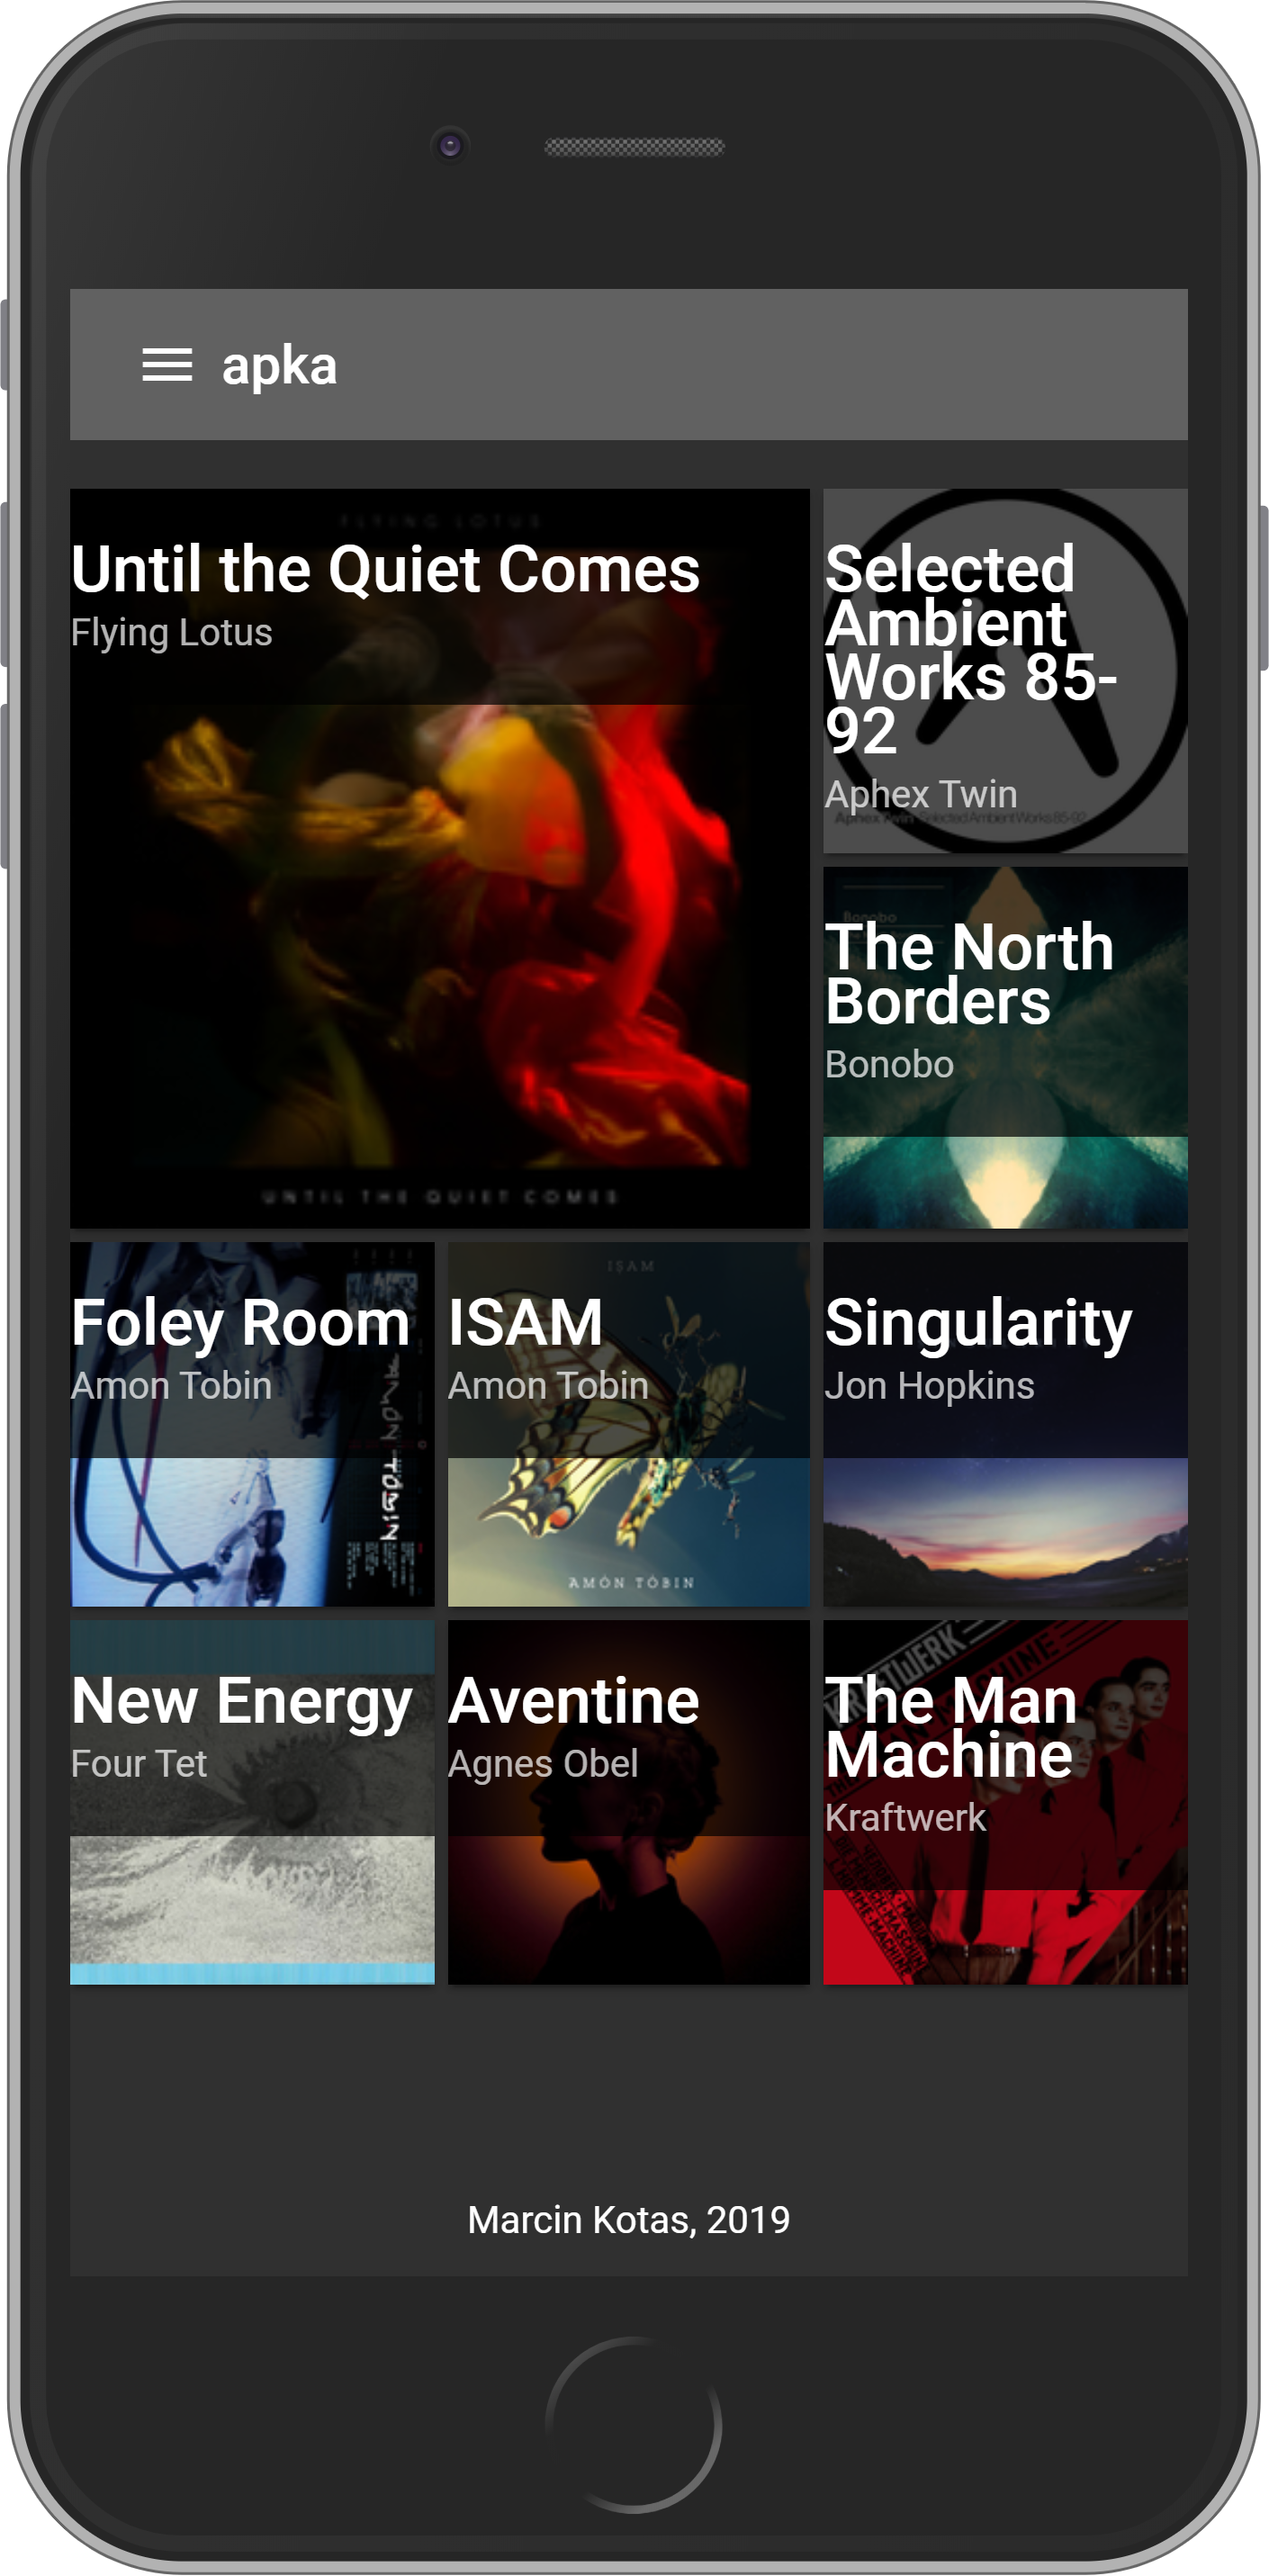
\includegraphics[width=0.75\linewidth]{rys07/explore.png}
			\caption{Widok wyświetlający listę albumów}
		\end{minipage}%
		\begin{minipage}{0.5\textwidth}
			\centering
			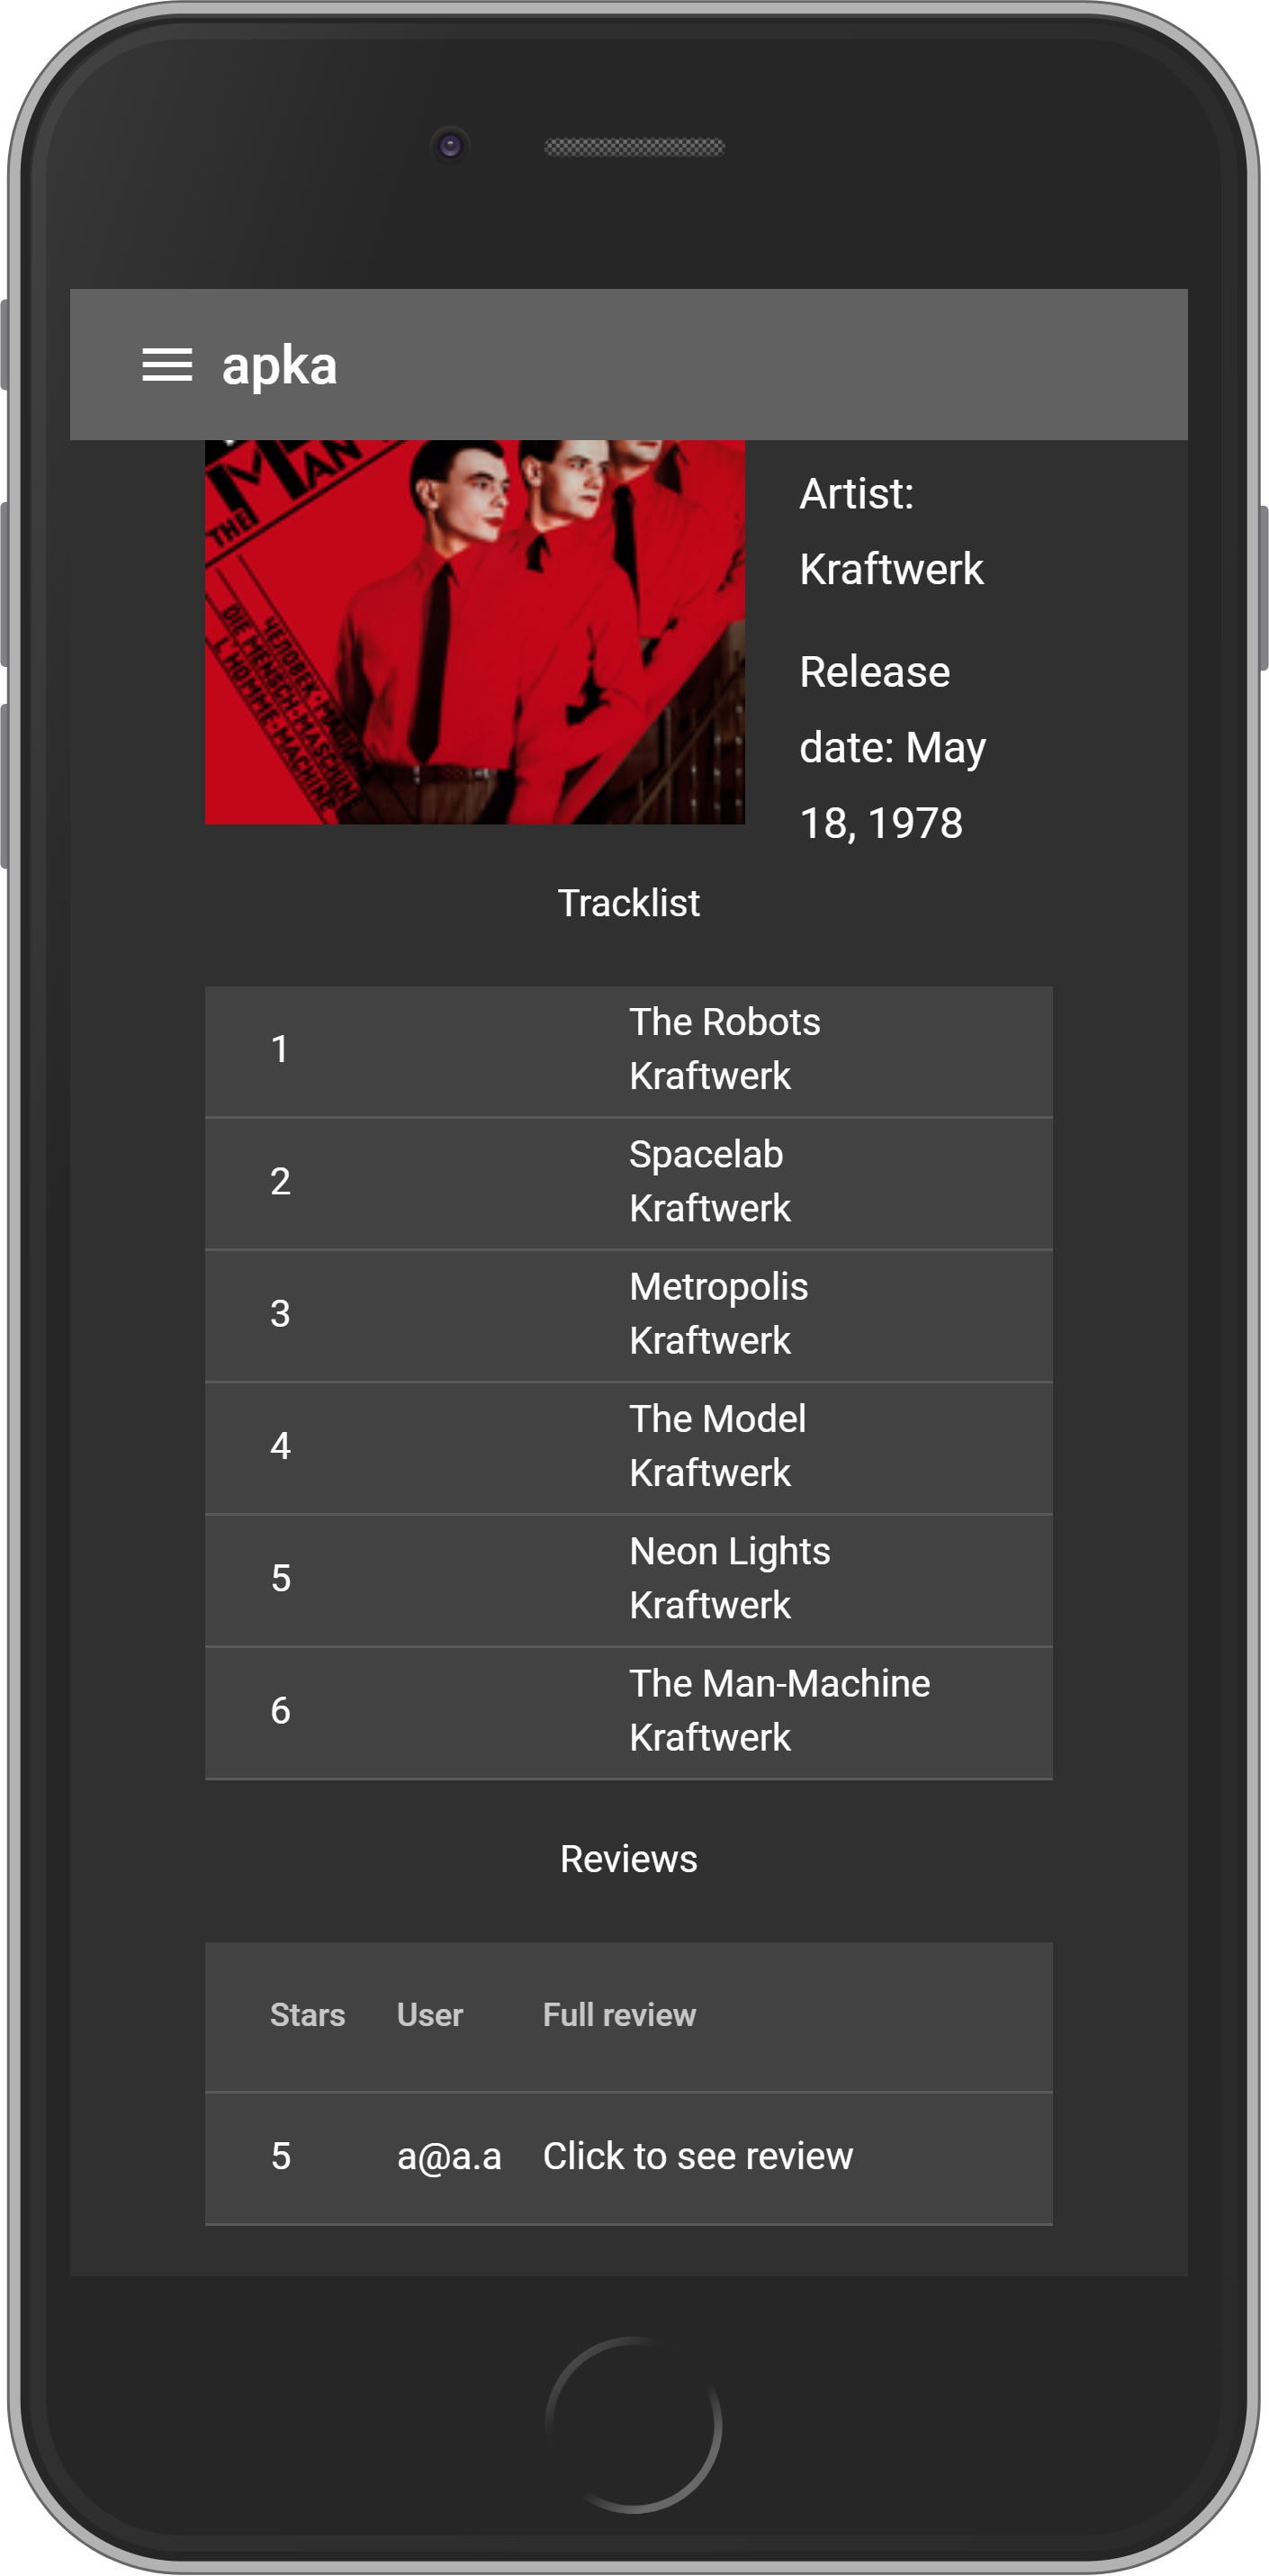
\includegraphics[width=0.75\linewidth]{rys07/album.png}
			\caption{Widok przedstawiający szczegóły albumu}
			\label{fig:album}
		\end{minipage}
	\end{figure}
	
\section{Dodawanie oceny}
	Dodawanie oceny odbywa się w dwóch krokach.
	Najpierw użytkownik wyszukuje album wg nazwy albumu, lub wpisuje nazwę artysty.
	W drugim przypadku zwracane są najpopularniejsze albumy danego artysty.
	Następnie, po kliknięciu w wybrany album użytkownik ma możliwość dodania oceny w skali 1-5 oraz opcjonalnie recenzji tekstowej (Rys.~\ref{fig:rate}).
	\begin{figure}[H]
		\centering
		\begin{minipage}{.5\textwidth}
			\centering
			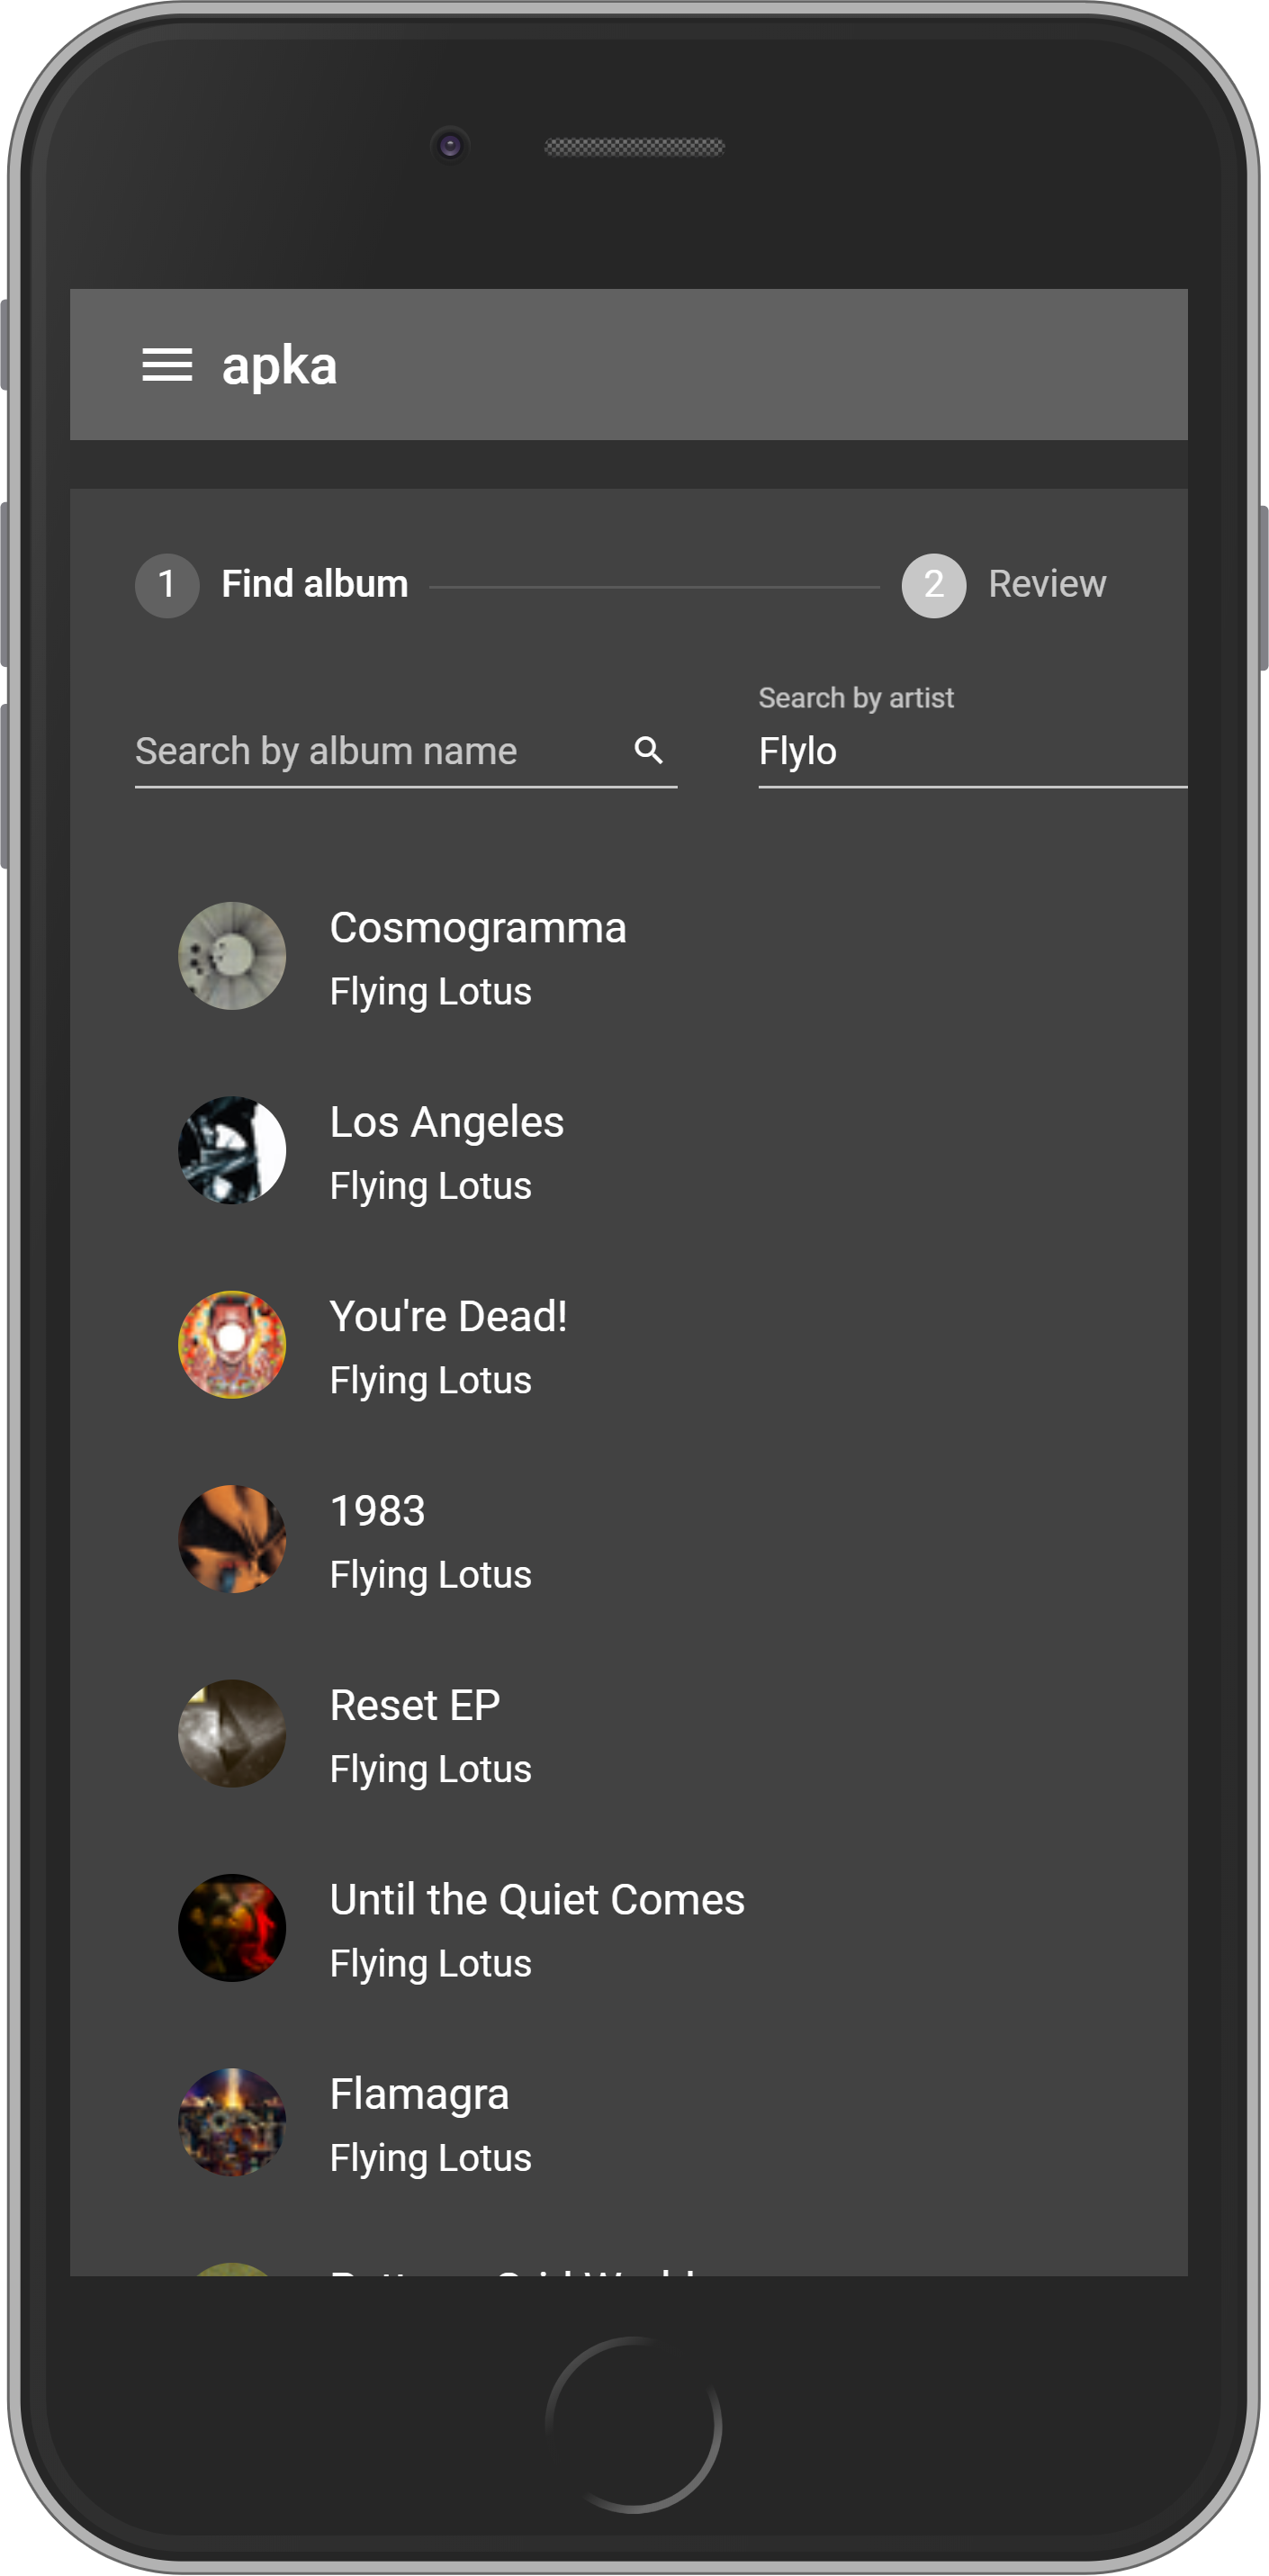
\includegraphics[width=0.75\linewidth]{rys07/search.png}
			\caption{Ekran wyszukiwania albumu}
		\end{minipage}%
		\begin{minipage}{0.5\textwidth}
			\centering
			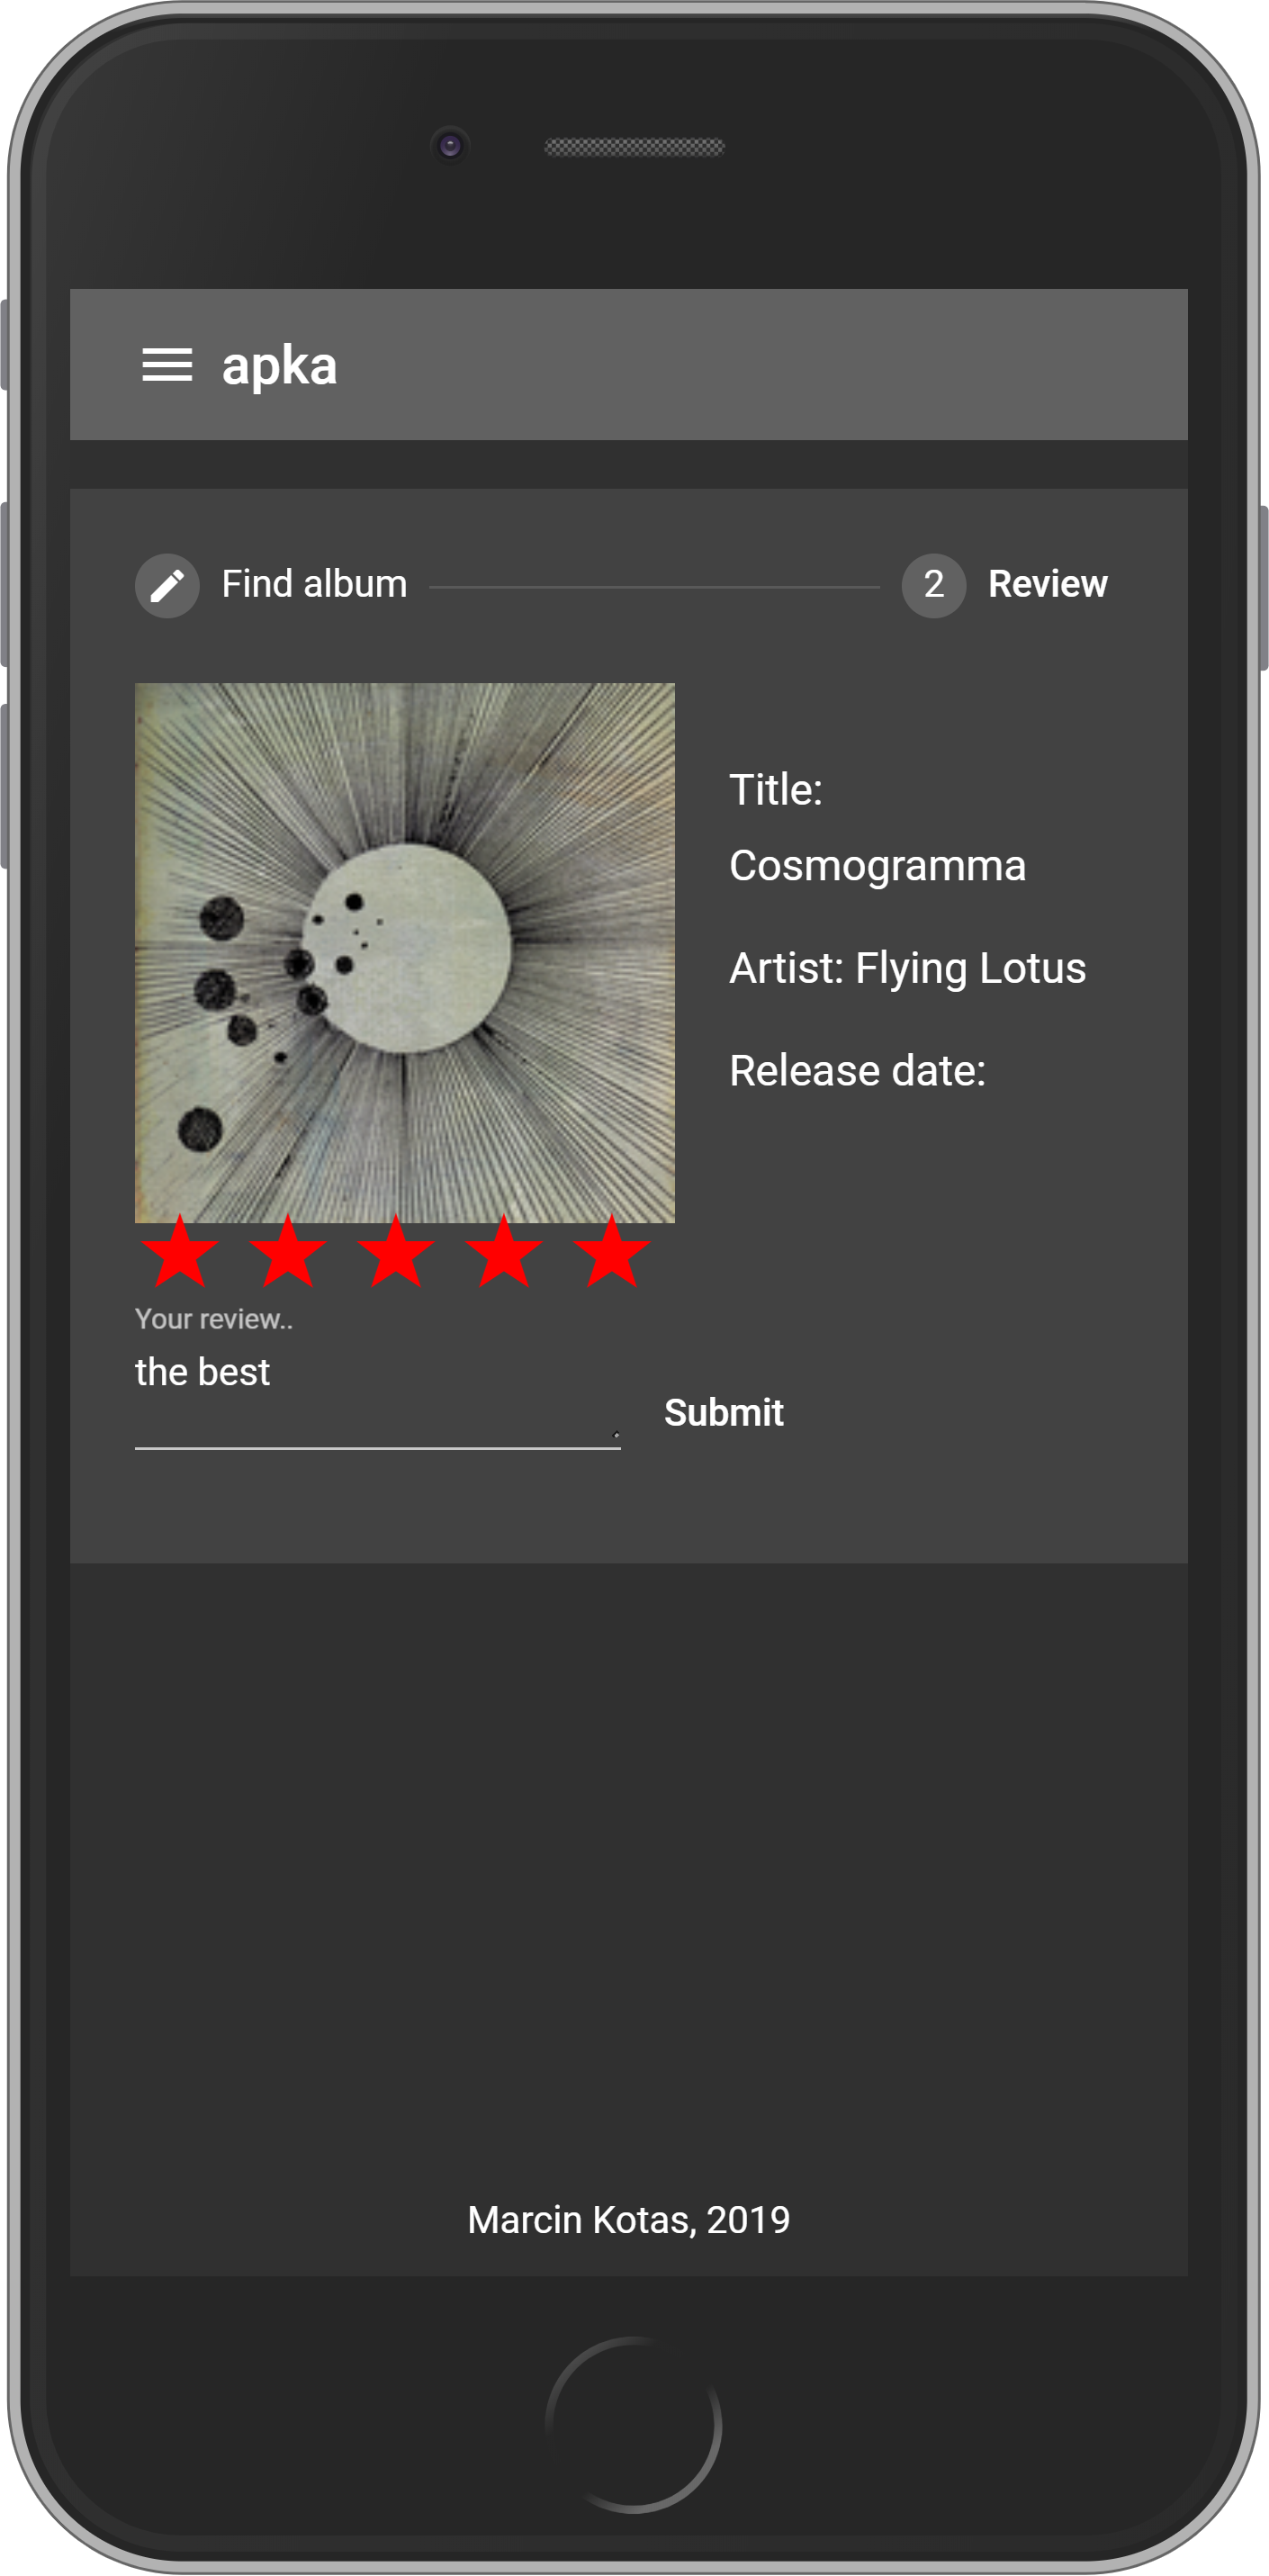
\includegraphics[width=0.75\linewidth]{rys07/rate.png}
			\caption{Ekrany dodawania oceny}
			\label{fig:rate}
		\end{minipage}
	\end{figure}

\newpage
\section{Rejestracja i logowanie}
	Zarówno rejestracja, jak i logowanie odbywa się po stronie serwisu Auth.
	Z tego powodu widoki te odstają stylistycznie od reszty aplikacji.
	\begin{figure}[H]
		\centering
		\begin{minipage}{.5\textwidth}
			\centering
			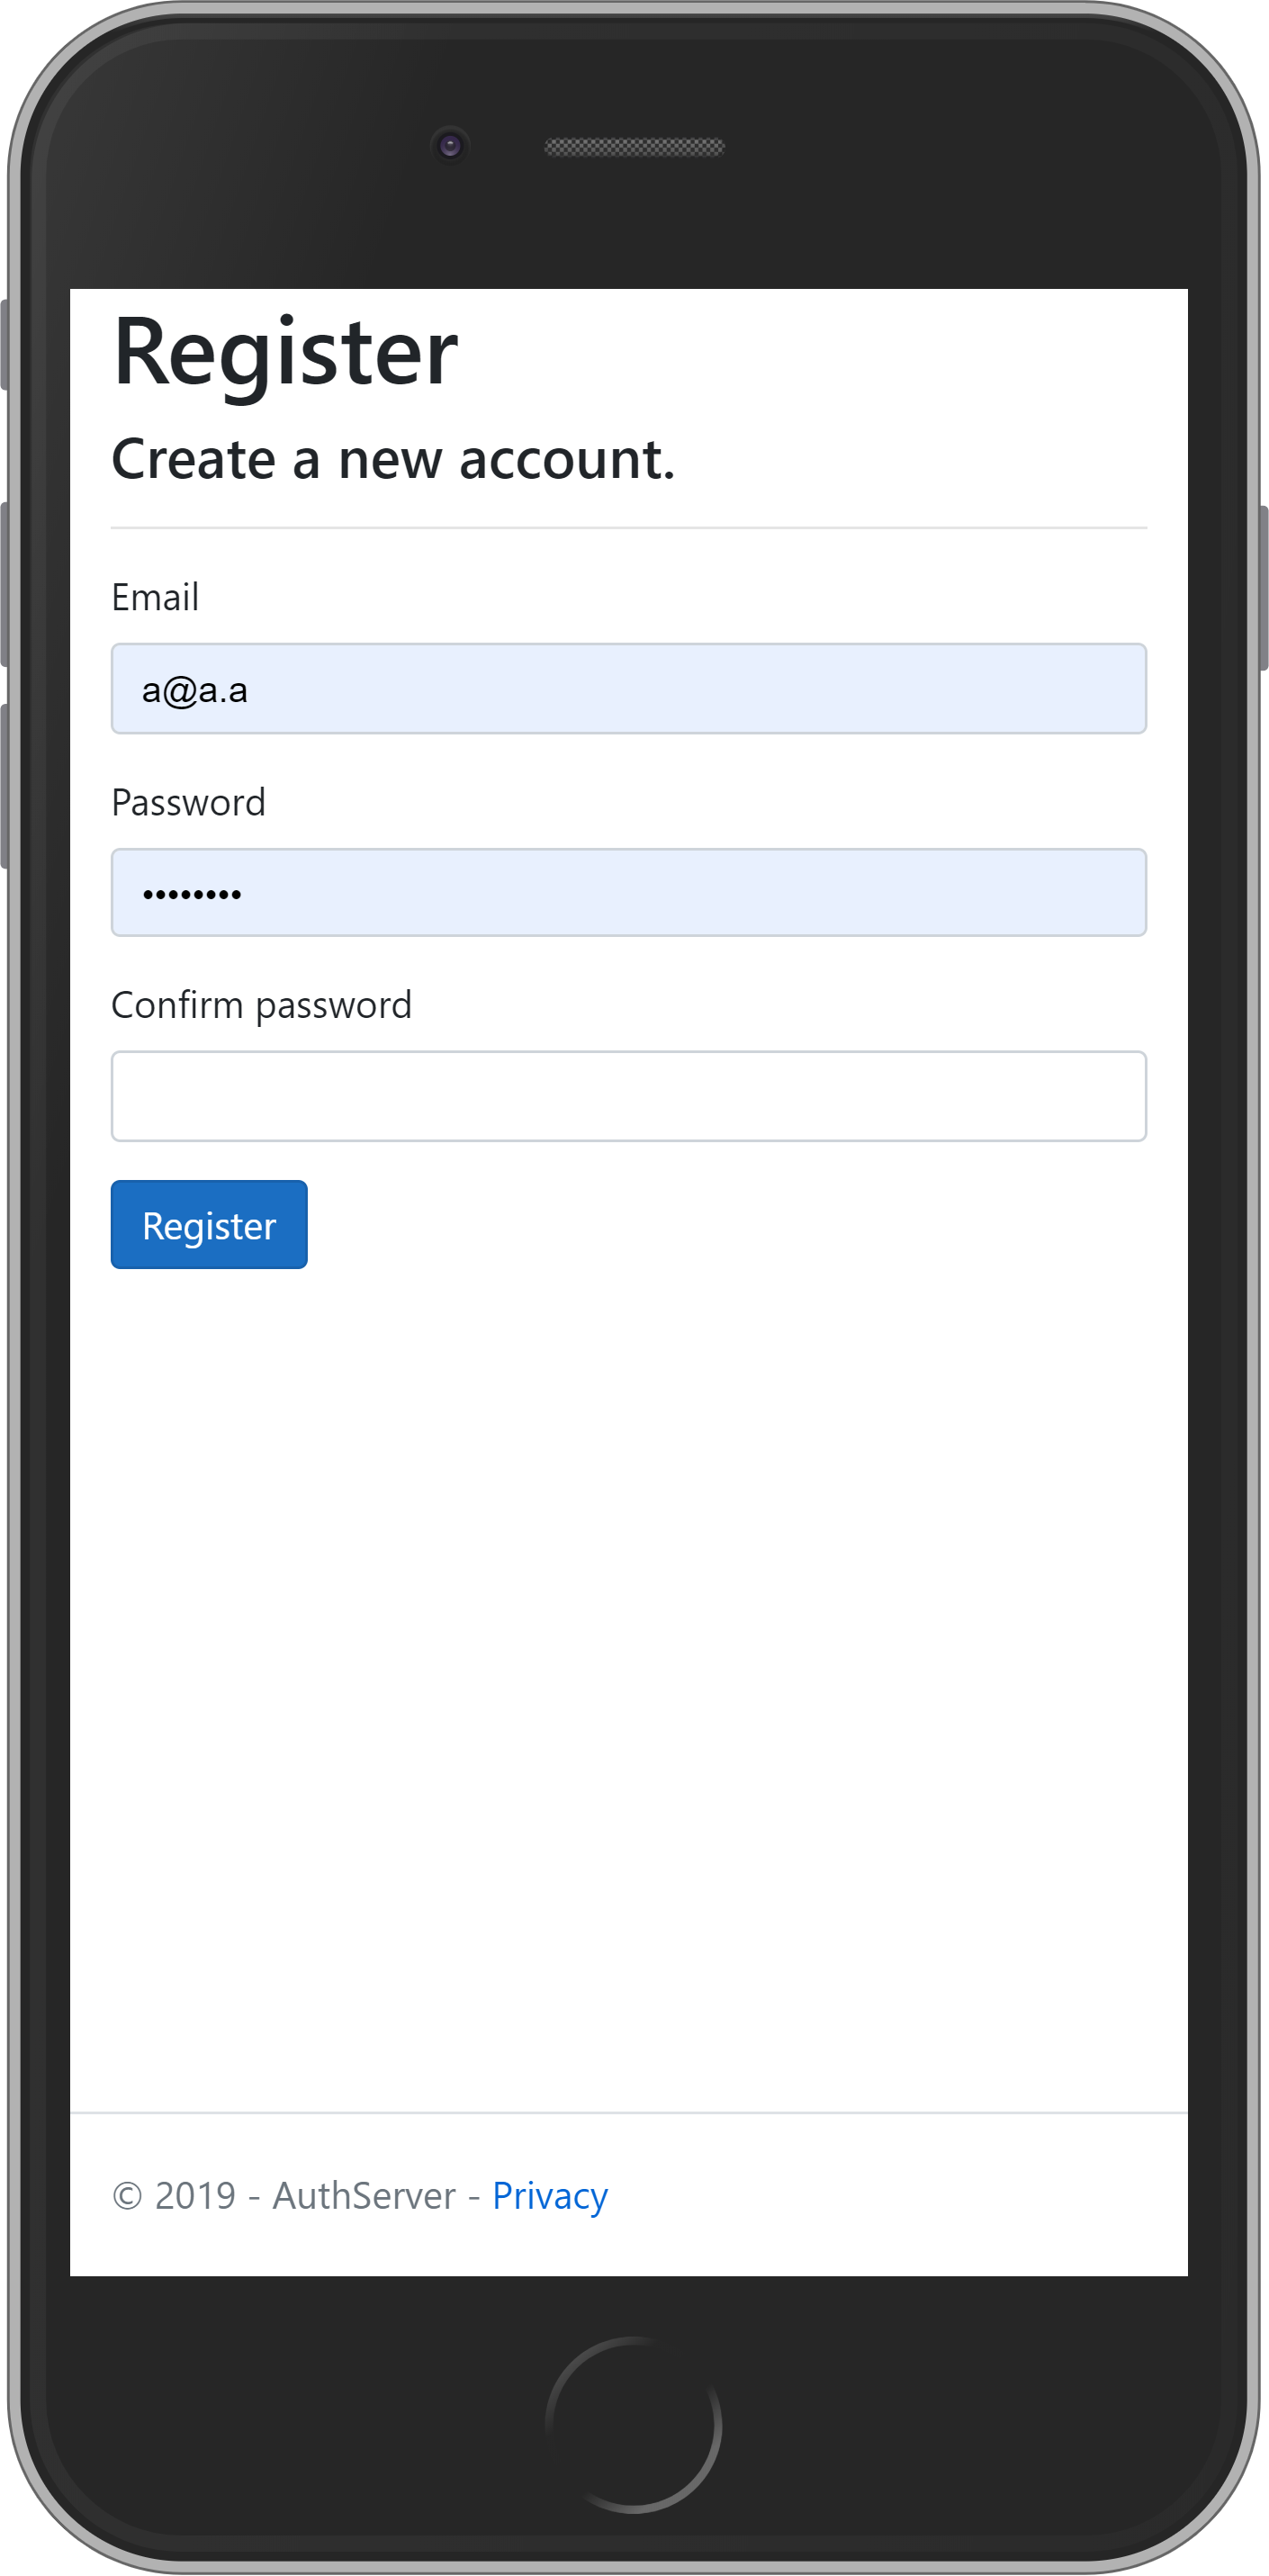
\includegraphics[width=0.75\linewidth]{rys07/register.png}
			\caption{Ekran rejestracji}
		\end{minipage}%
		\begin{minipage}{0.5\textwidth}
			\centering
			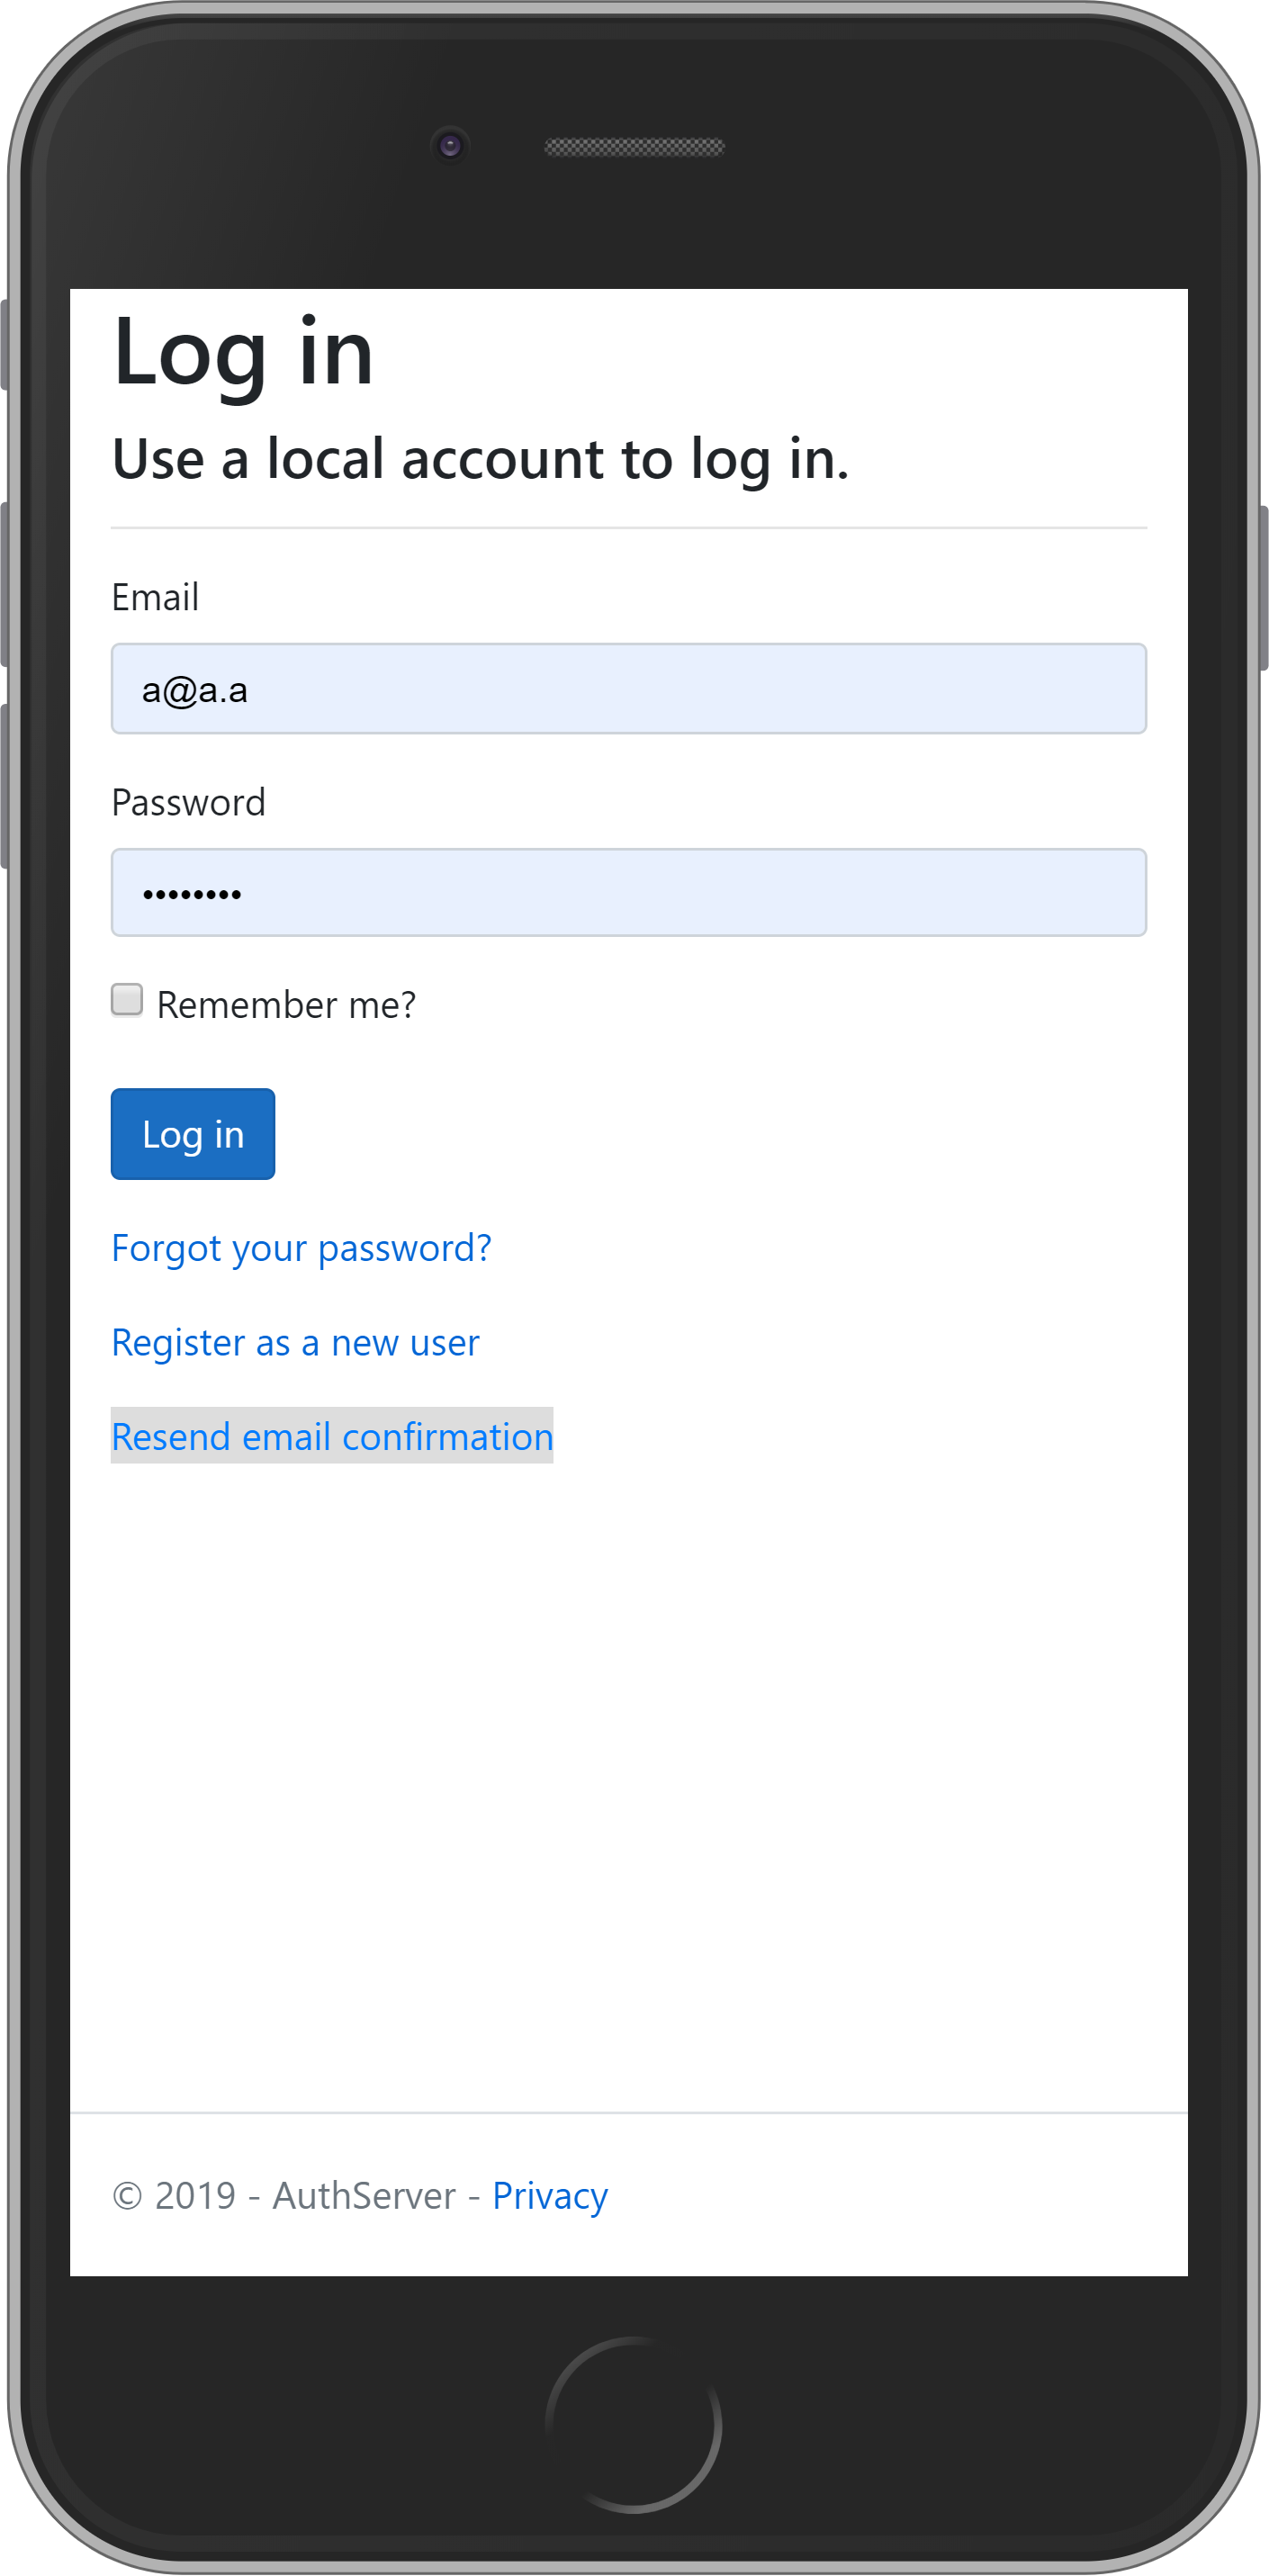
\includegraphics[width=0.75\linewidth]{rys07/login.png}
			\caption{Ekran logowania}
		\end{minipage}
		\label{fig:login}
	\end{figure}
	
\newpage
\section{Jasny motyw}
	Wszystkie widoki dostępne są również w jasnym motywie.
	Rysunek~\ref{fig:search_light} przedstawia wyszukiwanie po nazwie albumu,
	natomiast na rysunku~\ref{fig:album_light} przedstawiono widok~\ref{fig:album} w jasnym motywie.
	\begin{figure}[H]
		\centering
		\begin{minipage}{.5\textwidth}
			\centering
			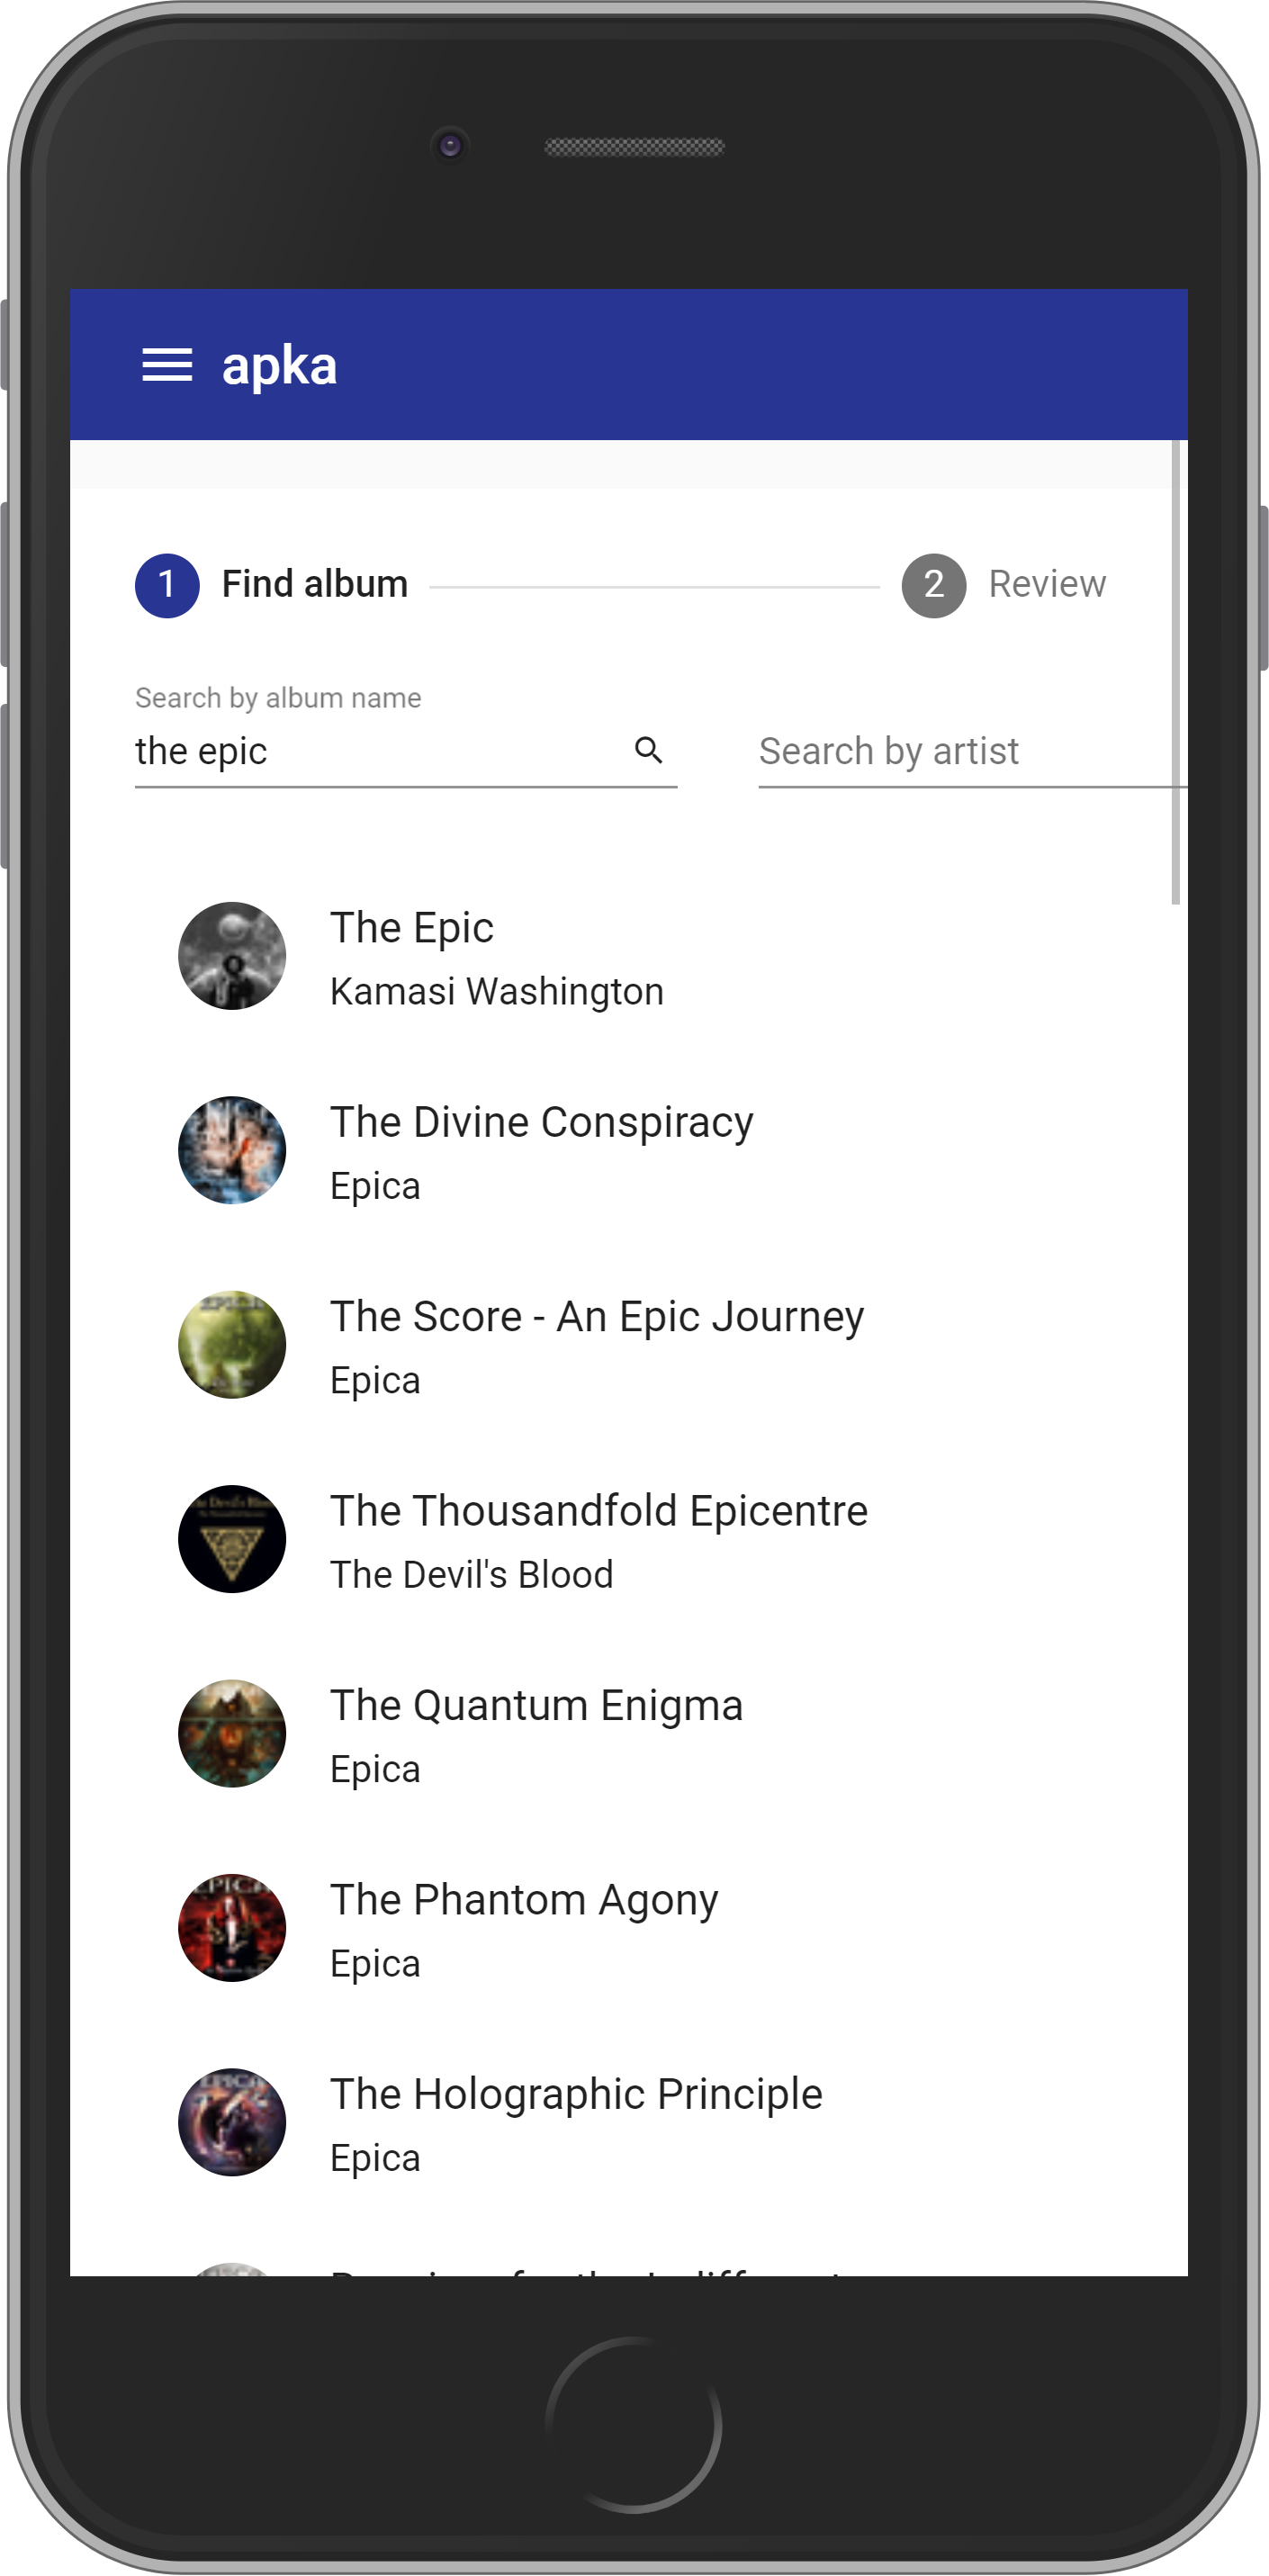
\includegraphics[width=0.75\linewidth]{rys07/search_light.png}
			\caption{Ekrany wyszukiwania albumu}
			\label{fig:search_light}
		\end{minipage}%
		\begin{minipage}{0.5\textwidth}
			\centering
			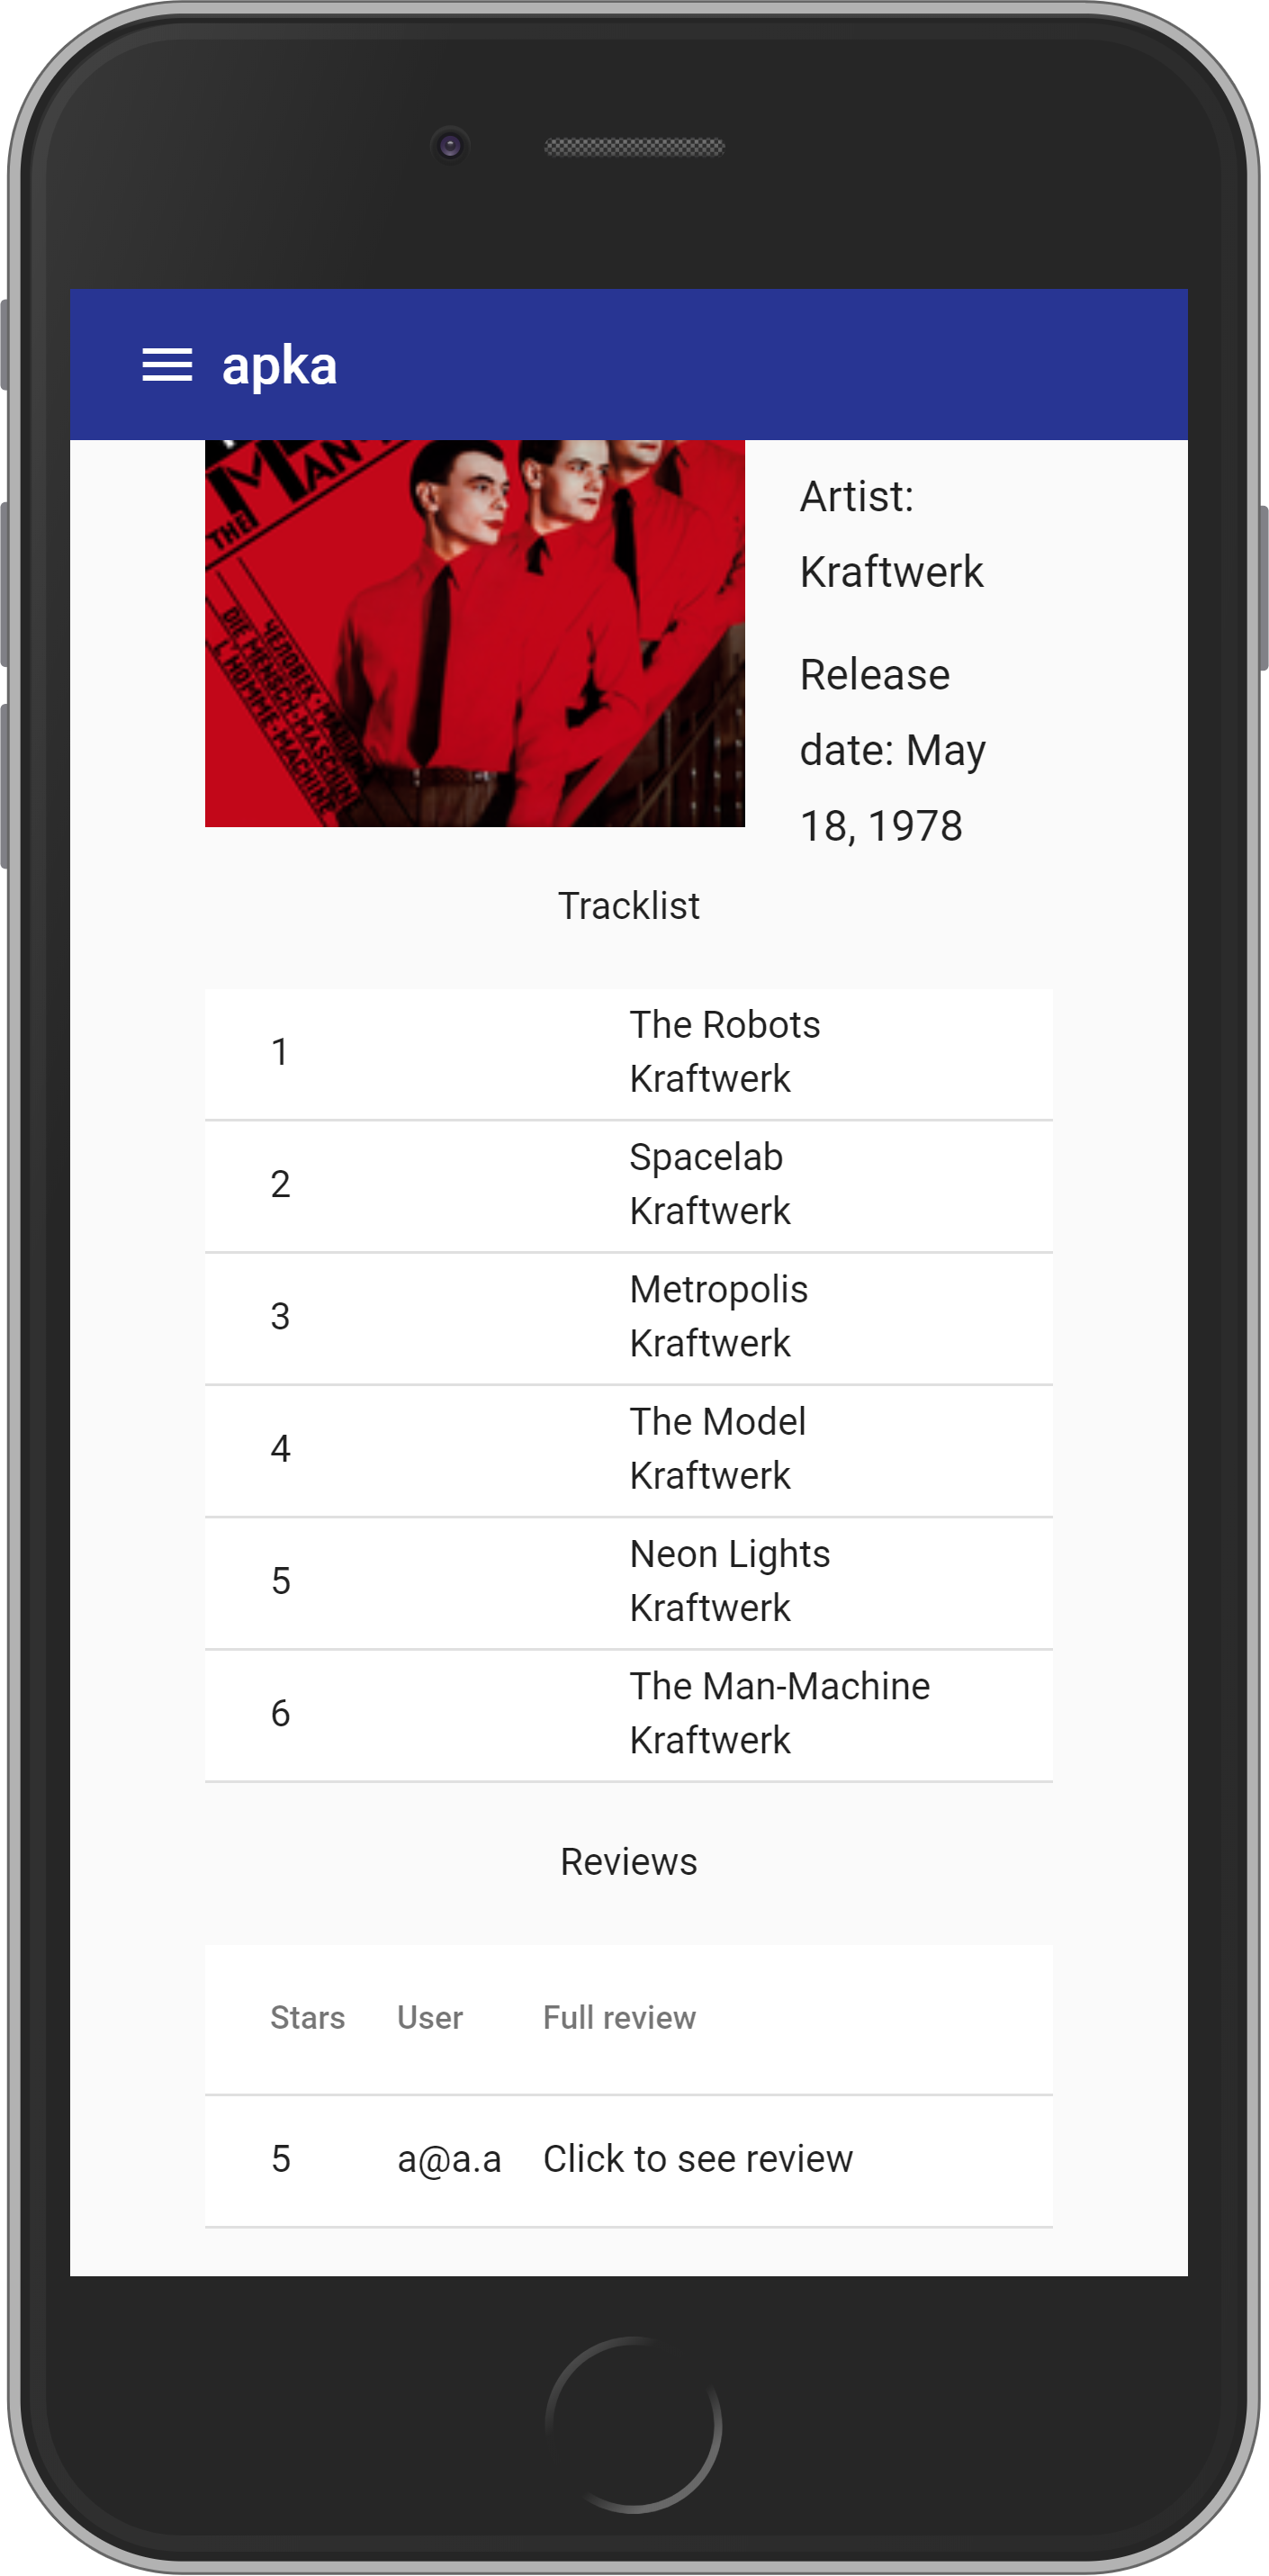
\includegraphics[width=0.75\linewidth]{rys07/album_light.png}
			\caption{Widok przedstawiający szczegóły albumu}
			\label{fig:album_light}
		\end{minipage}
	\end{figure}